\section{Prototype and Evaluation}
\label{sec:prototype}

% June 2016 high mempool: https://news.bitcoin.com/bitcoin-transactions-stuck/
% October 2016 high mempool: http://www.newsbtc.com/2016/10/27/new-bitcoin-mempool-backlog-crisis-averted-now/
% or t for top, b for bottom, h for here (https://tex.stackexchange.com/questions/35125/how-to-use-the-placement-options-t-h-with-figures)
%  - https://www.cryptocoinsnews.com/bitcoin-network-breaks-demand-surges/
\begin{figure*}[t]
	\centering
	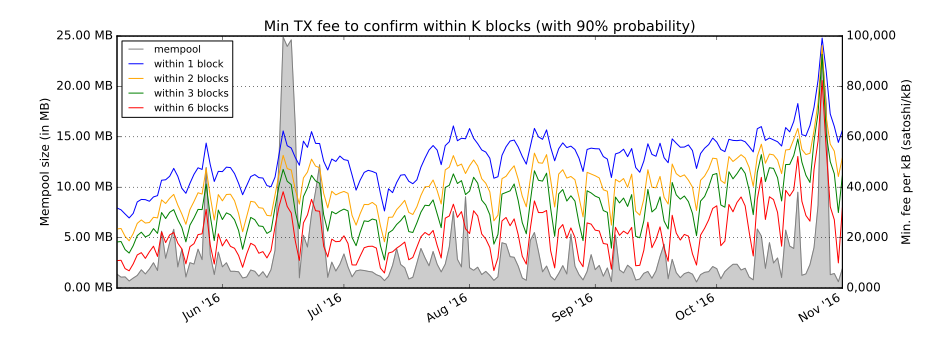
\includegraphics[width=2\columnwidth]{figs/txfee-estimates.eps}
	\vspace{-.9cm}
	\caption{This graphs shows the minimum transaction fee (in satoshi/kB) that guarantees a transaction will be included in the blockchain within $k$ blocks (for $k=1,2,3,6$) with 90\% probability (modeled using Feesim\cite{bitcoin-fees-github}). Fees tend to increase with contention for space in the Bitcoin ``mempool'' of unconfirmed transactions and transactions with higher fees get included in the blockchain faster. 1 satoshi = 0.00000001 BTC = $10^{-8}$ BTC and 1 kB = $10^3$ bytes.}
	\label{fig:fees}
\end{figure*}

We implemented a \Sys prototype in Java using the bitcoinj\cite{bitcoinj} library in 3000 lines of code, as measured with the \texttt{sloccount} tool.
Our code is available on GitHub: 

\begin{center}
\href{https://github.com/non-equivocation/catena-java}{\texttt{\footnotesize https://github.com/non-equivocation/catena-java}}
\end{center}

Our prototype implements a \Sys log server and a \Sys client, both operating as thin nodes on the Bitcoin network, but does not implement a header relay network (HRN).
Instead, in our first implementation, \Sys clients use only the Bitcoin P2P network to fetch both block headers and fetch \Sys transactions with their associated Merkle proofs.
In a future, more scalable implementation, we plan on fetching transactions and Merkle proofs from the log server and on using a header relay network for downloading block headers.
Next, we discuss our implementation and its internal API, which can be used to implement \Sys's API from \secref{sec:model:api}.

\subsection{\Sys Log Server}
The log server manages the statement key used to sign new \Sys statements (see \secref{sec:catena:design:transactions}) and a set of \emph{funding keys} used to ``re-fund'' a \Sys log (see \secref{sec:catena:design:refund}).
The server provides an $\mathsf{appendStatement(s)}$ API for issuing a statement $s$, which abstracts the Bitcoin layer away from applications.
Though currently not implemented, the server should ``re-fund'' the chain automatically assuming there are sufficient funds controlled by the funding keys.

\subsection{\Sys Log Client}
The client connects to the Bitcoin P2P network and sets a Bloom filter\cite{bloom} on all its connections to filter out irrelevant transactions.
This way, \Sys clients only receive server-issued \Sys transactions (see \secref{sec:background:bitcoin:thin}) and save orders of magnitude in bandwidth.
Recall that \Sys chains together transactions and clients verify this, thereby preventing malicious P2P nodes from equivocating about statements (see \secref{sec:catena:design:auditing}).
While additional bandwidth will be consumed by small blockchain reorganizations (see \secref{sec:catena:design:reorgs}), this amount should be negligible.

\Sys clients expose an $\mathsf{onStatementAppended(s)}$ API that notifies the higher level application of newly issued statements that have sufficient confirmations.
Applications are notified about statements in the order they were issued, making it easy to verify each statement for application-specific invariants (see \secref{sec:discussion:agnostic}).
If the \Sys log is caught equivocating, the \Sys client notifies the application via an $\mathsf{onEquivocation(s,s')}$ API that includes signatures on the two inconsistent statements $s$ and $s'$ and thus offers a publicly-verifiable non-repudiable proof of equivocation.

Certain applications might want to be made aware about the stability of Bitcoin's consensus.
For this, we provide an $\mathsf{onReorganize()}$ API that notifies applications about blockchain reorganizations with information about forks and the number of orphaned blocks.
Applications can use this information to infer whether the Bitcoin network is under attack, but we leave this to future work.

If bigger accidental or malicious forks should occur, they might unconfirm previously-confirmed \Sys transactions.
Even though such events are outside of our threat model, \Sys still notifies applications about statements that were unconfirmed via an $\mathsf{onStatementWithdrawn(s)}$ API so they can decide how to proceed.

\subsection{Costs and Overheads}

In this subsection, we discuss the financial cost of running a \Sys server, the overheads involved for clients and servers, and \Sys's scalability.

\subsubsection{Transaction Fees}
\label{sec:prototype:fees}
% https://bitcoinfees.21.co/#delay
% https://bitcoinfees.github.io/
% http://p2sh.info/dashboard/db/fee-estimation
Transaction fees in Bitcoin vary with contention for space in the blockchain (see \figref{fig:fees}) and so far have not been prohibitive for Bitcoin users.
For instance, Bitcoin transactions currently pay a fee of 70 satoshis per byte to get included in the blockchain within the next block\cite{bitcoin-fees-21co} (1 satoshi = $10^{-8}$ BTC).
For a 235-byte \Sys transaction that commits a statement consisting of a 256-bit SHA-256 hash, the fee would be 16,450 satoshis or 12 US cents per statement (on November 2016, 1 BTC = \$706.54).
If a statement is issued every 10 minutes, the cost per day would be less than 17.5 USD, which we believe is reasonable.
For example, this cost is not much higher than Keybase's cost\cite{keybase}, which issues statements less often (every 6 hours), paying a smaller fee of 10,000 satoshis or 7 US cents per transaction\cite{keybase-txs}.

\subsubsection{Overheads}
\label{sec:prototype:overheads}
\Sys's CPU overhead is insignificant.
A \Sys log server can issue at most one statement per Bitcoin block, so it only has to perform one signature every 10 minutes.
Similarly, \Sys clients only verify a transaction every 10 minutes for each log they audit, which adds virtually no overhead.
Finally, verifying the proof-of-work in block headers adds insignificant overhead.

\Sys clients need a small, constant amount of storage to recompute the Bitcoin difficulty and handle blockchain reorganizations.
To recompute the difficulty every 2016 blocks, \Sys clients and servers need to store the last 2016 block headers of the blockchain, which are 80 bytes each.
To prevent equivocation about withdrawn statements during blockchain reorganizations (see \secref{sec:catena:design:reorgs}), \Sys clients remember the past 100 statements issued by the server (no more than 80 bytes each due to \opret limits; see \secref{sec:background:bitcoin:opret}).
Here we assume that no Bitcoin fork, whether accidental or malicious, will be longer than 100 blocks.
Thus, \Sys's storage cost for both clients and servers is smaller than 200 KB.

\Sys demands a small amount of bandwidth from clients and a larger amount from servers who have to serve statements to clients.
First, servers and clients pay an initial cost to sync all the blockchain headers (currently \headerssize).
Servers and clients need to download all the headers so as to ensure the chain is sufficiently ``heavy'' and is thus the correct chain (see \secref{sec:background:bitcoin:consensus}).
Once this is done, \Sys clients need to sporadically connect to the header relay network to check for new block headers and connect to the log server to fetch new statements.
The required bandwidth for clients is less than 1 KB every 10 minutes: 600 bytes for statements and Merkle proofs and 80 bytes for each block header, possibly requested from multiple HRN nodes.
In contrast, the server needs bandwidth linear in the number of \Sys clients, since it serves every statement to each client.

\subsubsection{Scalability}
We believe \Sys can scale easily if the header relay network distributes block headers and the \Sys log server distributes statements and proofs.
However, our current implementation based on Bitcoin's P2P network will not scale beyond tens of thousands of \Sys clients without putting significant stress on Bitcoin.
As discussed in \secref{sec:catena:design:header-relay}, there simply aren't enough connections available in the Bitcoin network to support a large number of \Sys clients.
In addition, our current implementation relies on disk-intensive Bloom filtering (see \secref{sec:background:bitcoin:thin}).
We stress that these are current, surmountable limitations of Bitcoin that all \emph{thin} blockchain-based applications need to deal with, not just \Sys.

\subsection{Preventing Equivocation in CONIKS}
\label{sec:prototype:coniks}

\newcommand{\numlinessv}{66\xspace}
\newcommand{\numlinescl}{89\xspace}

To demonstrate \Sys's applicability to key transparency schemes, we modified CONIKS\cite{coniks} to publish directory digests in a \Sys log so as to prevent a malicious provider from equivocating about its \pkd.
Our modified CONIKS is as hard to fork as Bitcoin, which we believe makes CONIKS more resilient to attacks.
Our changes to CONIKS are minimal, consisting of \numlinessv new lines of code for the CONIKS server and \numlinescl new lines of code for the CONIKS test client. (We changed Java source files, project files and configuration files.)

A typical CONIKS provider advertises the root hash of a prefix Merkle tree periodically to CONIKS clients.
This root hash is signed and is referred to as a Signed Tree Root (STR).
To prevent impersonation, clients have to gossip STRs amongst themselves or with different providers.
Our modification of CONIKS removes the need for gossiping by witnessing STRs in the Bitcoin blockchain using a \Sys log.
This allows all CONIKS clients to agree on the same history of STRs.
We lowered the frequency at which providers publish STRs from once per minute to once per ten minutes to coincide with the frequency of Bitcoin blocks.
We also modified the CONIKS test client to listen for Bitcoin-witnessed STRs.
However, because the provided test client is not fully implemented to keep track of STRs, more changes to CONIKS, not \Sys, are needed to actually prevent equivocation.

\Sys does not change CONIKS's public-key distribution assumptions.
CONIKS assumes that clients have a way of obtaining the public keys of providers.
Similarly, our Bitcoin-witnessed CONIKS assumes that clients have a way of obtaining the ``public keys'' for the \Sys logs of providers.
Specifically, our ``public key'' is the log's genesis transaction (see \secref{sec:catena:design:genesis}).
We commit the old public key of the provider in the auxiliary data of the genesis transaction (see \secref{sec:model:api}).
CONIKS clients need this public key to verify CONIKS server replies to their queries.